\section{Design of the Wah-Wah Effect}

\subsection{Choice of the Bandpass Filter}

The block diagram of the wah-wah effect has been presented in the analysis and is shown again below in  \autoref{fig:wah_diag_2}:

\begin{figure} [htbp]
	\centering
	\begin{picture}(0,0)%
	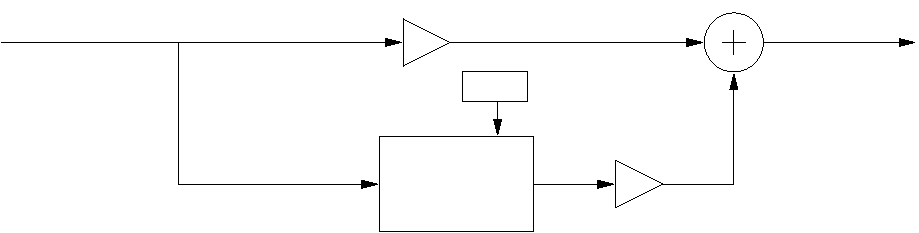
\includegraphics{wah_diag.pdf}%
	\end{picture}%
	\setlength{\unitlength}{4144sp}%
	%
	\begingroup\makeatletter\ifx\SetFigFont\undefined%
	\gdef\SetFigFont#1#2#3#4#5{%
		\reset@font\fontsize{#1}{#2pt}%
		\fontfamily{#3}\fontseries{#4}\fontshape{#5}%
		\selectfont}%
	\fi\endgroup%
	\begin{picture}(6999,1770)(2689,-2233)
	\put(6841,-1591){\textit{Wah-Wah Gain}}%
	\put(5626,-2041){$Filter$}%
	\put(6136,-1186){\textit{LFO or Pedal}}%
	\put(2746,-646){$Input$}%
	\put(8686,-646){$Output$}%
	\put(5626,-1816){$Bandpass-$}%
	\put(5986,-646){$Gain$}%
	\end{picture}%
	\caption{Block diagram of the wah-wah effect}
	\label{fig:wah_diag_2}
\end{figure}

In signal processing, different types of filters can be implemented using the first and second order allpass filters. In the case of the wah-wah, it can be inferred from \autoref{fig:wah_diag_2} that a bandpass filter is need where the center frequency is controller in order to choose where the filter is working in the frequency spectrum. \\

With a first order allpass filter, it is possible to design a circuit to make  lowpass and highpass filter but not bandpass or bandreject. Thus, the focus will be on the second order allpass filter since a bandpass one is needed. \\

\autoref{fig:wah_allpass} shows the block diagram of the second order allpass filter.

\begin{figure} [htbp]
	\centering
	\begin{picture}(0,0)%
	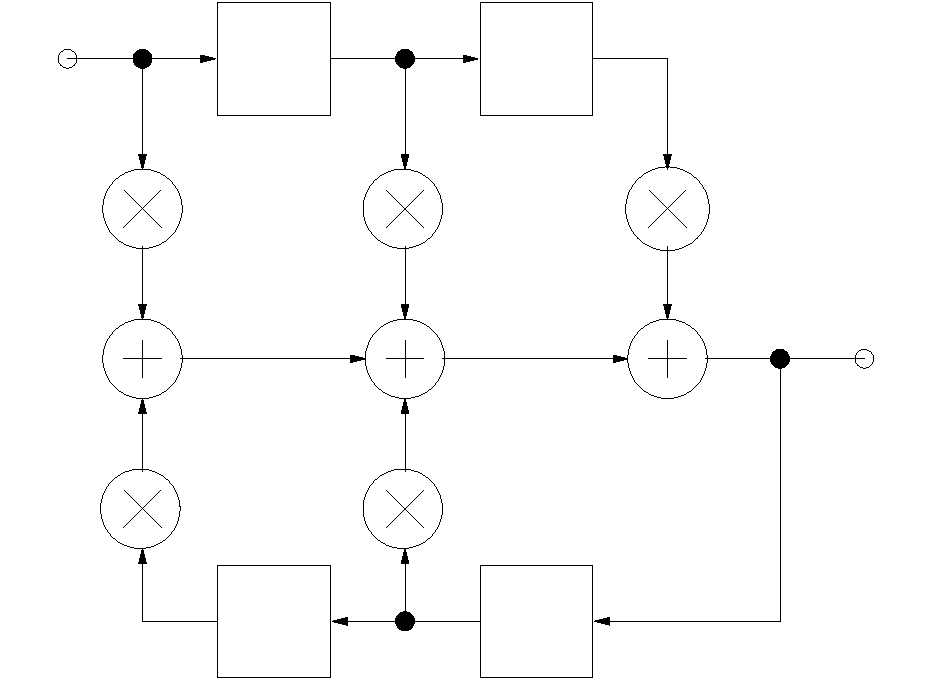
\includegraphics{wah_allpass.pdf}%
	\end{picture}%
	\setlength{\unitlength}{3947sp}%
	%
	\begingroup\makeatletter\ifx\SetFigFont\undefined%
	\gdef\SetFigFont#1#2#3#4#5{%
		\reset@font\fontsize{#1}{#2pt}%
		\fontfamily{#3}\fontseries{#4}\fontshape{#5}%
		\selectfont}%
	\fi\endgroup%
	\begin{picture}(7524,5424)(1411,-5923)
	\put(3001,-2236){-c}%

	\put(3526,-1036){T}%

	\put(5626,-1036){T}%

	\put(5626,-5536){T}%
	
	\put(3526,-5536){T}%
	
	\put(8551,-3436){y(n)}%
	
	\put(1426,-1036){x(n)}%
	
	\put(4426,-811){x(n-1)}%
	
	\put(6451,-811){x(n-2)}%
	
	\put(2251,-5686){y(n-2)}%
	
	\put(4426,-5761){y(n-1)}%
	
	\put(7201,-2236){1}%
	
	\put(3001,-4636){c}%
	
	\put(5101,-4636){-d(1-c)}%
	
	\put(5101,-2236){d(1-c)}%
	
	\end{picture}%
	\caption{Block diagram for a second-order allpass filter \citep{DAFX}}
	\label{fig:wah_allpass}
\end{figure}

The transfer function in Z-domain can be inferred from \autoref{fig:wah_allpass} :

\begin{equation} \label{wah_z_equation}
		A(z) = \frac{-c+d(1-c)z^{-1}+z^{-2}}{1+d(1-c)z^{-1}-cz^{-2}}
		\end{equation}
		
where:

\begin{equation}
	c = \frac{tan(\pi f_{b}/f_{s})-1}{tan(\pi f_{b}/f_{s})+1}
	\end{equation}

and

\begin{equation}
	d = -cos(2\pi f_{c}/f_{s})
	\end{equation}

$f_{s}$ represents the sampling frequency, $f_{c}$ the cutoff frequency and $f_{b}$ the ??. The factor $d$ grants control over the cutoff frequency while the factor $c$ permits the change in bandwidth. \\

From the \autoref{wah_z_equation}, it is possible to obtain the equation in the discrete time-domain that can then be used for digital implementation which includes Matlab simulations and so on. 
\begin{equation}\label{wah_eq_1}
	y(n) = -cx(n) + d(1-c)x(n-1) + x(n-2) - d(1-c)y(n-1) + cy(n-2)  
\end{equation}


Using the allpass filter presented above, it is possible to create a bandpass filter by simply summing the input signal with the one coming from the allpass filter, a block diagram that illustrates the design for a better understanding is in \autoref{fig:wah_bandpass}:

\begin{figure} [htbp]
	\centering
	\begin{picture}(0,0)%
	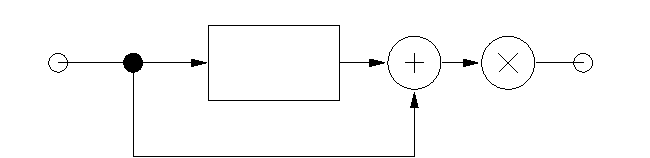
\includegraphics{wah_bandpass.pdf}%
	\end{picture}%
	\setlength{\unitlength}{3947sp}%
	%
	\begingroup\makeatletter\ifx\SetFigFont\undefined%
	\gdef\SetFigFont#1#2#3#4#5{%
		\reset@font\fontsize{#1}{#2pt}%
		\fontfamily{#3}\fontseries{#4}\fontshape{#5}%
		\selectfont}%
	\fi\endgroup%
	\begin{picture}(5199,1257)(3136,-2923)
	\put(5926,-2011){\textit{y(n)}}%
	
	\put(5176,-2236){\textit{A(z)}}%
	
	\put(7051,-1861){\textit{1/2}}%
	
	\put(3050,-2236){$x_{b}(n)$}%
	
	\put(7951,-2236){$y_{b}(n)$}%
	
	\put(4276,-2011){\textit{x(n)}}%
	
	
	\end{picture}%
	
	\caption{Block diagram for a second-order bandpass filter \citep{DAFX}}
	\label{fig:wah_bandpass}
\end{figure}

From \autoref{fig:wah_bandpass}, the transfer function of the bandpass filter is then:

\begin{equation}
 	H(z) = 1/2 (1 + A(z))
\end{equation}

The discrete time equation can also be inferred:

\begin{equation}\label{wah_eq_2}
		y_{b} = \frac{1}{2} (x(n) + y(n))
\end{equation}

since $y(n)$ is known from \autoref{wah_eq_1}, \autoref{wah_eq_2} can be re-written as :

\begin{equation}
			y_{b}(n) = \frac{1}{2} ((1-c)x(n) + d(1-c)x(n-1) + x(n-2) - d(1-c)y(n-1) + cy(n-2) )
\end{equation}


\section{Bandpass filter using Chamberlin}

\autoref{fig:wah_bandpass_second} shows the general topology of the Chamberlin state variable filter.

\begin{figure} [htbp]
	\centering
	\begin{picture}(0,0)%
	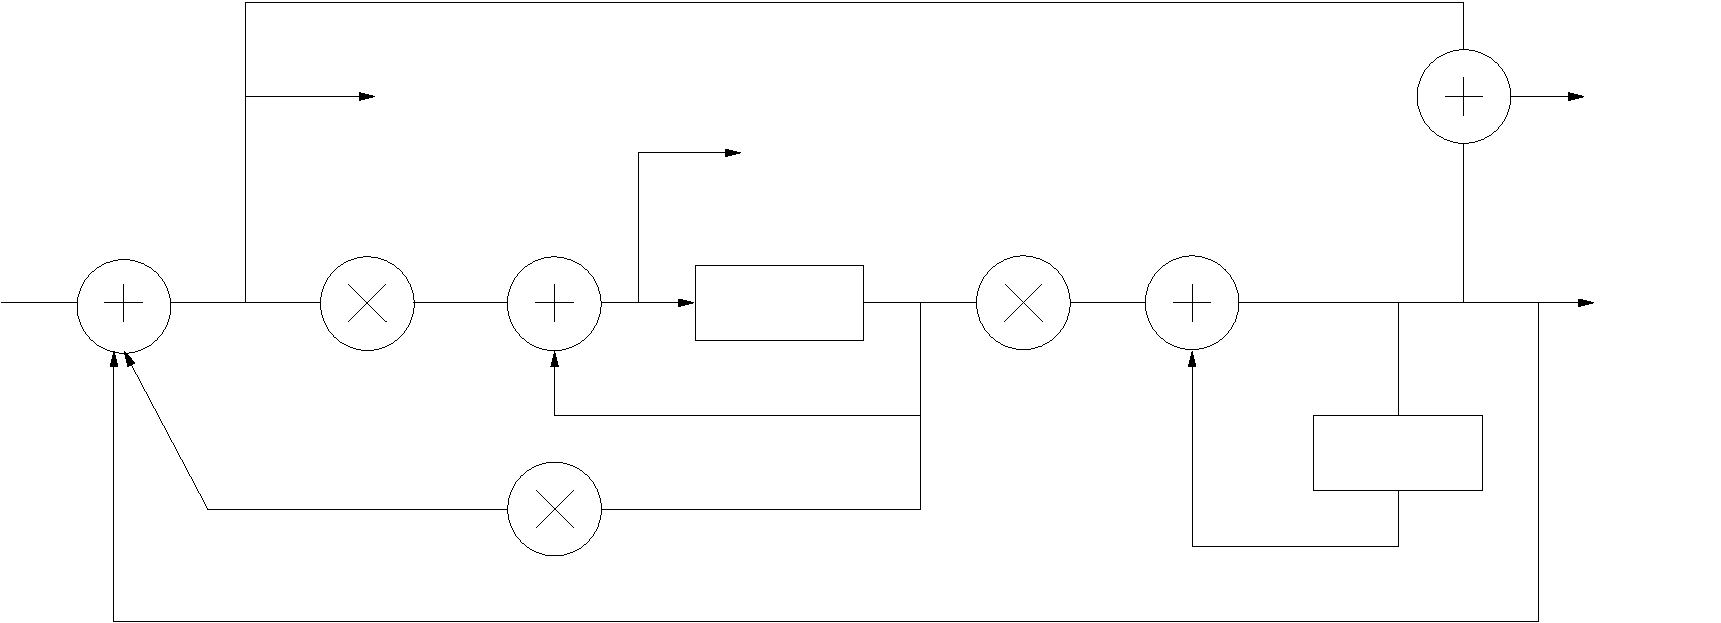
\includegraphics[width=1\textwidth]{wah_bandpass_second.pdf}%
	\end{picture}%
	\setlength{\unitlength}{1973sp}% un scaled 3947sp
	%
	\begingroup\makeatletter\ifx\SetFigFont\undefined%
	\gdef\SetFigFont#1#2#3#4#5{%
		\reset@font\fontsize{#1}{#2pt}%
		\fontfamily{#3}\fontseries{#4}\fontshape{#5}%
		\selectfont}%
	\fi\endgroup%
	\begin{picture}(13761,4974)(139,-5173)
	\put(826,-3186){\textit{-}}%
	
	\put(6001,-2786){$z^{-1}$}%
	
	\put(10951,-3986){$z^{-1}$}%
	
	\put(3226,-950){\textit{Highpass}}%
	
	\put(6076,-1436){\textit{Bandpass}}%
	
	\put(12976,-2636){\textit{Lowpass}}%
	
	\put(12901,-1086){\textit{Bandreject}}%
	
	\put(9600,-2161){\textit{f}}%
	
	\put(3000,-2161){\textit{f}}%
	
	\put(4501,-3811){\textit{q}}%
	
	\put(1426,-3186){\textit{-}}%
	
	\end{picture}%
	
	
	\caption{Block diagram the Chamberlin state variable filter topology \citep{}}
	\label{fig:wah_bandpass_second}
\end{figure}

This topology can be used to obtain a bandpass filter with a variable center frequency. 

The factor $f$ that is shown on \autoref{fig:wah_bandpass_second} is the frequency control coefficient defined as in the following equation:

\begin{equation}
      f = 2 \cdot sin(\frac{\pi \cdot f_{c}}{f_{s}})
\end{equation}

The factor $q$ is defined as the inverse of the Q-factor.

\begin{equation}
			q = \frac{1}{Q}
\end{equation}

The minimum value for the Q-factor is normally 0.5 while the maximum value of the frequency control coefficient $f$ is 1. 


\begin{comment}
sources:
http://www.earlevel.com/main/2003/03/02/the-digital-state-variable-filter/
\end{comment}